%%% Local Variables:
%%% mode: latex
%%% TeX-master: "../main"
%%% coding: utf-8
%%% End:
% !TEX TS-program = pdflatexmk
% !TEX encoding = UTF-8 Unicode
% !TEX root = ../main.tex

This section discusses the results, and experience gained by implementing a project using WebGPU in detail. In addition, a discussion of the results is provided and possible future work is outlined.

The path tracer focuses on the given use case and is therefore not a general-purpose rendering engine. For example, it does not offer a physics engine, support for animations, or other features that are common in general-purpose rendering engines such as \gls{Three.js}, \gls{Babylon.js} or alternatives. Generally, the ray tracing technique is slower than rasterization-based approaches and is therefore not a silver bullet for all use cases. Yet, for the given use case of using production \gls{CAD} data with manifold assembly configurations and customer-specific materials, the path tracer is a suitable choice. This makes it a viable option in the case of e-commerce. Additionally, operating costs can be reduced by eliminating the need to host a rendering pipeline or remote rendering service. WebGPU has significant potential for years to come and adoption of \gls{OpenPBR} by the wider industry is a promising sign of the possible longevity of the chosen technology and standards.

\section{Comparison to Prior Work}

The three existing open-source path tracers for the web are alternatives to the renderer developed in this work. While comparing them based on quantitative measures such as \fGls{FPS}{\e{Frames per second}, measure of rate at which consecutive images are rendered and displayed} is not meaningful as the number of samples differs across the renderers, it is still possible to define a set of criteria to compare them.


\subsection*{WebGPU Support}

WebGPU is a new technology and support for it is likely to become more important in the future. The three alternatives currently do not support WebGPU and still rely on \gls{WebGL}.

\subsection*{PBR Standard}

As discussed in \autoref{ch:materialDescriptionStandards}, a variety of standards exist for \gls{PBR}. While \gls{OpenPBR} is a new standard, it has already seen adoption by the industry. \texttt{three-gpu-pathtracer} and \texttt{Three.js PathTracer} currently use custom \gls{PBR} standards or partially support \gls{glTF} PBR extensions. \texttt{dspbr-pt} uses the \gls{DSPBR} standard.

\subsection*{Documentation}

In order to be usable by developers, the renderer should be well-documented. \texttt{strahl} and \texttt{three-gpu-pathtracer} provide documentation. \texttt{Three.js PathTracer} and \texttt{dspbr-pt} provide minimal documentation.

\subsection*{npm Package}

The availability of an \gls{npm} package can simplify the integration of the renderer into existing projects. \texttt{strahl}, \texttt{three-gpu-pathtracer}, and \texttt{dspbr-pt} provide an \gls{npm} package. \texttt{Three.js PathTracer} does not provide a package.

\subsection*{Last Update}

The last update of the renderer is an indicator of the activity of the project. \texttt{strahl}, \texttt{three-gpu-pathtracer}, and \texttt{Three.js PathTracer} have been updated in 2024. \texttt{dspbr-pt} has not been updated since 2022.

\subsection*{Assessment}
\autoref{tab:rendererComparison} contains a high-level comparison between the four renderers. The renderer developed in this work is the only one that supports WebGPU and uses the \gls{OpenPBR} standard. The renderer is also available as an \gls{npm} package and provides an alternative to the existing renderers.

\begin{table}[H]
    \centering
    \ra{1.3}
    \begin{tabular}{@{}p{3cm}p{2.5cm}p{2.5cm}p{2.5cm}p{2.5cm}@{}}
    \toprule
     & \texttt{strahl} & \texttt{three-gpu-} \texttt{pathtracer} \cite{ThreeJsPathTracerJohnson} & \texttt{Three.js PathTracer} \cite{ThreeJsPathTracerLoftis} & \texttt{dspbr-pt} \cite{PathTracerDassault} \\
    WebGPU \newline Support & Yes & No & No & No \\
    \gls{PBR} Standard & \gls{OpenPBR} & Custom & Custom & \gls{DSPBR} \\
    Documentation & yes & yes & minimal & minimal \\
    \gls{npm} Package & yes & yes & no & yes \\
    Last Update & 2024 & 2024 & 2024 & 2022 \\
    \bottomrule
    \end{tabular}
    \caption{High-level comparison between the four open-source path tracers for the web.}
    \label{tab:rendererComparison}
  \end{table}

\section{Findings}

The main novelty introduced in this work is the development of a path tracer with WebGPU using the \gls{OpenPBR} surface shading model. WebGPU and \gls{OpenPBR} are promising endeavors for the future of 3D rendering, but relatively new and not yet widely adopted.

\subsection*{State of WebGPU}

As highlighted in the report, WebGPU is a promising technology for \gls{GPGPU} computations in the browser. However, to date there are certain limitations in terms of support and features.

\subsubsection*{Browser Support}

Due to the current state of support for WebGPU in Safari and Mozilla Firefox, the production readiness of WebGPU is still limited. Safari has announced plans to support WebGPU and has launched a preview version \cite{SafariWebGPUSupport}. Firefox also has plans to support WebGPU \cite{FirefoxWebGPUSupport}. Thanks to the extensive conformance test suite \cite{WebGPUConformanceTestSuite}, it is more likely that the different implementations will be compatible with each other.

The main browser which supports WebGPU to date is Chrome. WebGPU has shipped to general use on desktops in May of 2023 \cite{ChromeWebGPUSupport}. Since January 2024, WebGPU is also supported on modern Android devices \cite{ChromeAndroidWebGPUSupport}.

This means that it's straightforward to use WebGPU on most modern devices with the notable exception of Apple iOS and iPadOS devices.

\subsubsection*{Ray Tracing}

To date, WebGPU does not support some features that are common in modern rendering \glspl{API} and would be beneficial for the path tracer. The most prominent example is hardware-accelerated ray tracing. \glspl{API} such as Vulkan support hardware-accelerated ray tracing \cite{vulkanRayTracing}. This entails helpers for building common acceleration structures, such as \gls{BVH}, as well as ray querying functions to determine intersections. WebGPU does not yet support these features, but there are discussions ongoing to add extensions \cite{webGPURayTracing} as well as a demonstration implemented in a Dawn fork \cite{webGPURayTracingFork}.

\subsubsection*{Debuggability}

None of the major browser engines, Chrome, Firefox, and Safari, provide debugging as part of the developer tools. Tools for inspecting WebGPU applications exist \cite{webGpuDevToolsDuncan, webGpuDevToolsTakahiro}, but are limited in terms of feature set. While they are helpful to inspect the pipelines, capture frames, and inspect resources, they do not provide debugging capabilities such as breakpoints, stepping or variable inspection. For specific setups, there are methods to setup profiling \cite{webGpuProfilingWithPix}, but these are not integrated into the browser developer tools and are dependent on the concrete machine hardware. Improvements in this area would be beneficial for productivity.

\subsubsection*{Stability}

To date, there are reports of stability issues with WebGPU. This includes crashes of the browser, but on macOS using Chrome system-wide crashes have been observed with faulty WebGPU code. Such issues can look like shown in \autoref{fig:webgpu-crash}. Due to the early stage of the technology and the complexity of the underlying system, such stability issues ought to be expected. As implementations mature, these issues are likely to be resolved.

\begin{figure}[H]
  \centering
  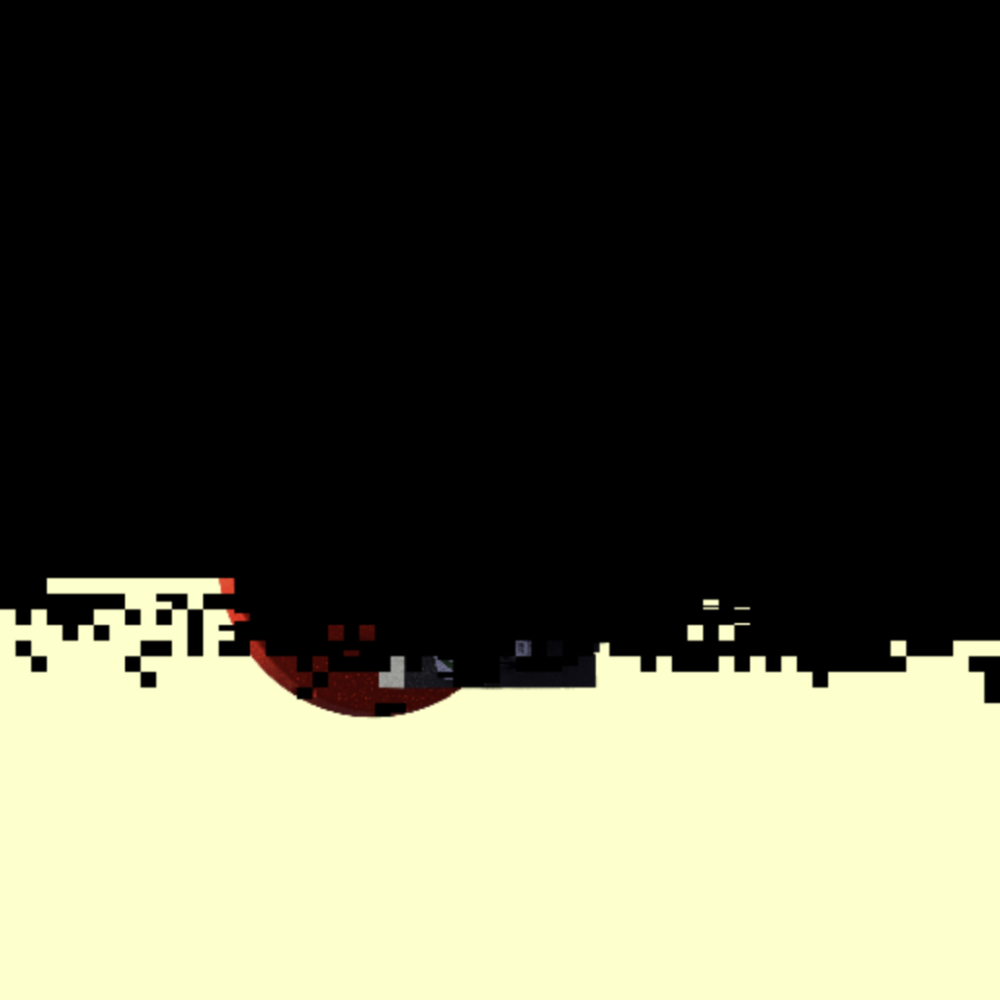
\includegraphics[width=0.25\columnwidth]{resources/webgpu-crashes.png}
  \caption{Example of a provoked WebGPU crash on macOS, note the black squares which correspond in size to the dispatched workgroup size.}
  \label{fig:webgpu-crash}
\end{figure}

\subsection*{OpenPBR}

The integration of the \gls{OpenPBR} surface shading model enables realistic material representation. As it is a new standard and no stable version has been released when first implementing the path tracer, aligning it with the standard was challenging. To date only few open-source projects have implemented the standard. Since the standard has reached a stable version during the work on this thesis, aligning effort between the implementation and the standard has reduced. The use of \gls{PBR} and the latest industry standards is beneficial and provides good quality results. The adoption track of \gls{OpenPBR} is promising and the standard is likely to be extended in the future.

\section{Future Work}

In order to accomodate for other use cases, the renderer could be extended in various ways. The following section outlines possible future work which includes extending \gls{PBR} capabilities, improving performance, extending to other rendering architecture paradigms, general improvements for the WebGPU community, and aligning the renderer with other standards.

\subsection*{Rendering Effects}

The focus on the defined use case means that certain rendering effects are not implemented. These include:

\begin{itemize}
    \item{Refraction}.
    \item{Caustics}.
    \item {Depth of Field} - Depth of field is the effect of objects at different distances from the camera being in focus or out of focus.
    \item {Motion Blur} - Motion blur is the effect of objects moving quickly appearing blurred.
    \item{Volumetric Effects}.
    \item{Hair and Fur}.
\end{itemize}

While refraction, caustics, depth of field, and motion blur are a question of light transport, volumetric effects, hair and fur are features that are not part of the \gls{OpenPBR} specification.

\subsection*{Spectral Rendering}

Instead of the \gls{RGB} color space, spectral rendering uses the full spectrum of visible light by modeling the light as a function of wavelength. This can improve the realism of the rendered images. Spectral rendering is well-suited for \gls{PBR} and is therefore a natural extension of the current implementation. It is also possible to support both \gls{RGB} and spectral rendering.

\subsection*{Texture Support}

While not critical for the given use case, texture support is a common feature in rendering engines. The current implementation does not use textures. THe renderer could be extended to support sampling \gls{OpenPBR} parameters from textures. This would enable more complex material variations and possibly improve the realism of the rendered images.

This should not be confused with texture mapping frequently used in rasterization-based rendering engines. Texture mapping is a technique to apply images to surfaces to simulate surface details. In path tracing, textures are used to sample material properties such as base color, roughness, or metallicness.

\subsection*{Full OpenPBR support}

The current implementation only supports the features of the \gls{OpenPBR} surface shading model that are required for the given use case. The full \gls{OpenPBR} specification includes additional features that could be implemented to improve the realism of the rendered images. These include:

\begin{itemize}
    \item{Subsurface Scattering} - Subsurface scattering is the effect of light entering a surface and being scattered beneath the surface before exiting at a different point. This effect is common in materials such as skin, wax, or marble.
\end{itemize}

\todo{list all features}

\subsection*{Alignment of OpenPBR and glTF PBR}

Further improvements can be achieved by aligning \gls{glTF} PBR with \gls{OpenPBR}, focusing on real-time rendering. This alignment could reduce the computational resources required for surface shading.

\subsection*{Web Worker Support}

Web Workers are a web technology that allows running scripts off the main thread. This can be used to offload \gls{CPU}-heavy tasks to a separate thread to prevent blocking the main thread which is responsible for rendering the user interface.

\subsection*{BVH Construction}
\label{sec:bvhConstructionDiscussion}

The current implementation builds the \gls{BVH} on the \gls{CPU} and transfers it to the \gls{GPU}. Corresponding research \cite{lauterbach2009GPUbvh} suggests that moving parts of the construction to the \gls{GPU} directly could improve performance. This would reduce the amount of data that needs to be transferred between the \gls{CPU} and the \gls{GPU}. The new \gls{GPGPU} capabilities of WebGPU further enable this approach.

\subsection*{TypeScript Support for Memory Management}

While \texttt{webgpu-utils} \cite{webgpuUtilsLib} is useful for memory management, it does not provide TypeScript support for the generated definitions based on the underlying \gls{WGSL} code. Type safety could reduce the likelihood of errors in the code. As an alternative, runtime checks could be implemented to ensure that the data is correctly mapped to all fields of the underlying structure.

\subsection*{Independence of Three.js}

For ease-of-use for developers, the renderer is using \gls{Three.js} helpers. This aids developers familiar with \gls{Three.js} to get started with the renderer as configuration for scene loading and camera configuration is similar. However, the renderer does not depend on \gls{Three.js} and could be used independently. The main drawback of the dependence is the increased bundle size. Possibly, \texttt{three-mesh-bvh} \cite{threeMeshBvh} could also be exchanged for an alternative library or self-implemented as described in \autoref{sec:bvhConstructionDiscussion}. By removing the dependency, the bundle size could be reduced. To support developers, a binding to \gls{Three.js} could be provided on top of the independent renderer.

\subsection*{Offline and Remote Rendering}

As highlighted in \autoref{ch:paradigmAssessment}, it is possible to extend a real-time client side renderer to be used in offline and remote rendering scenarios. In order to implement offline rendering, one could opt to use a headless browser such as Puppeteer, a \fgls{Node.js}{JavaScript runtime, frequently used for executing JavaScript outside of the browser} library which provides a high-level \gls{API} to control browsers. An alternative is to use \gls{wgpu}, but this would necessitate a rewrite of the renderer. Possibly, the rewritten renderer could also be used in the web context by using \fgls{WebAssembly}{Portable Binary-code format for executable programs available in modern browser engines}.

For remote rendering, the renderer could be extended to render images on demand and encode them as video streams.

\subsection*{WebGPU Compatibility Mode}

There is a proposal under active development which aims to extend the reach of WebGPU by providing a slighly restricted subset of WebGPU \cite{WebGPUCompatibilityModeProposal}. Considering the suggested limits of the compatibility mode, it could be possible to deploy the renderer onto a wider range of devices. However, it is important to consider that path tracing is a computationally expensive task and might not be suitable for all devices. Therefore, increasing the reach might not be beneficial in all cases.

\subsection*{Automatic Shader Conversion}

During the specification phase of WebGPU, the relation to \fgls{SPIR-V}{\e{Standard Portable Intermediate Representation}, intermediate language for parallel computing and graphics developed by Khronos Group} was discussed \cite{webGPUSpirVRelation}. In general, many of the modern shading languages can be compiled to one another. Projects such as Tint, which is part of \gls{Dawn} \cite{dawnImplementation} or Naga \cite{nagaImplementation} could be used to compile shaders from different frontends to different backends. Similarly, other engines such as \gls{Three.js} with \fGls{TSL}{\e{Three.js Shading Language}, shading language used in \gls{Three.js} which supports \gls{GLSL} as well as \gls{WGSL}} have their own shading languages which support a variety of backends \cite{ThreeJSShadingLanguage}. Parts of \gls{MaterialX} shader generation could be used to generate shaders for WebGPU and update them automatically as \gls{OpenPBR} is updated.

\subsection*{Low-Level Performance Optimizations}

This target is likely at odds with the goal of providing automatic shader generation. The current implementation is not optimized for performance. Therefore, it is likely that optimizations of the \gls{WGSL} code could improve the performance of the renderer. Due to the nature of the design of \gls{OpenPBR}, it would be possible to do optimizations and get better real-time rendering performance.

Automatic shader generation is helpful, but likely not as optimized as a carefully tuned implementation. However, both endeavors are of interest for potential benefits.

\subsection*{Sampling Performance Optimizations}

Path tracing is computationally expensive and requires multiple samples per pixel to achieve accurate results. Consequently, the sampling process is noticeable during interactions with the scene. One technique to improve perceived interaction quality is to overlay the rendering with a rasterization preview during interactions. To reduce the number of samples required for higher quality renderings, techniques like neural radiance caching (NRC) \cite{muller2021real} or reservoir-based spatio-temporal importance resampling (ReSTIR) \cite{restir} could be employed in future work.

\subsection*{Denoisers}

Optimizations in the render pipeline could also be achieved by using denoising algorithms applied as post-processing steps could enhance the quality of the results. Options include blockwise multi-order feature regression (BMFR) \cite{blockwise-multi-order-regresssion-for-rt-pt} and Open Image Denoise (OIDN) \cite{openImageDenoise}.

\subsection*{Qualitative Assessment}

The provided results highlight the quantitative performance of the renderer. However, due to the nature of a renderer, qualitative assessment based on visual inspection is also used to determine the quality of the rendered images. This could be extended to include more advanced metrics such as peak signal to noise ratio (PSNR), structural similarity (SSIM) \cite{ssim}, or learned perceptual image patch similarity (LPIPS) \cite{lpips}.

Such a comparison could be based on reference scenes such as the Cornell Box \cite{goral1984modeling} or the Sponza Atrium \cite{dabrovic2002sponza}. To assess the differences, a number of tests could be conducted:

\begin{itemize}
    \item{Offline Renderer Comparison} - Comparison to other offline renderers such as Cycles \cite{cycles}, Mitsuba \cite{Jakob2020DrJit} or \gls{pbrt} \cite{Pharr_Physically_Based_Rendering_2023}.
    \item{Rasterization Renderer Comparison} - Comparison to rasterization-based web renderers such as \gls{Three.js} or \gls{Babylon.js}.
    \item{Web-based Path Tracer Comparison} - Comparison to other web-based path tracers such as \texttt{three-gpu-pathtracer} \cite{ThreeJsPathTracerJohnson}, \texttt{Three.js PathTracer} \cite{ThreeJsPathTracerLoftis}, or \texttt{dspbr-pt} \cite{PathTracerDassault}.
\end{itemize}


\subsection{ReSTIR}
\subsection{SHaRC}

https://intro-to-restir.cwyman.org/